% g-2 Introduction
\chapter {Introduction}

In particle physics, \gmtwo of the muon, and \gmtwo in general, is an important and deep probe into the Standard Model (SM). The gyromagnetic ration, $g$, represents the coupling strength of a particle to the type of helicity flipping transitions mediated by magnetic fields, and the $\hbox{--}2$ portion denotes the subtraction of the expected value of the gyromagnetic ratio, leaving only the anomalous magnetic moment, $a$.  The quantities acts as both a seed for new particle physics models and a scythe on proposed models.   Contributions to the quantity depend on the gamut of fundamental interactions and constants of the universe in the SM: quantum electrodynamics (QED), Weak and Strong interactions all playing important roles.  Precision measurement of \gmtwo facilitates development of standard model extensions of somewhat analogous interactions of particles inspired by SM particles. 

\section{History}

For many years the value of both $g_e$ and $g_\mu$ were thought to be exactly $2$ as predicted for pure Dirac particles\cite{the-muon-g-2}. And, initial experiments supported the prediction that $g = 2$ \todo{cite initial expt}. That notion, however, had to be reconciled with experiment as measurement precision progressed and statistical tensions arose with the values predicted by theory.  Deviations from a pure Dirac particle were first observed in hyperfine splitting measurements of several different nuclei.  The measured deviations were not statistically significant until Kusch and Foley measured the atomic spectra of several nuclei in 1947 \cite{kusch-foley}.  The theory community quickly resolved the discrepancy with a now standard QED calculation of the lowest order self-interaction for leptons emitting and reabsorbing photons, see figure \ref{fig:schwinger-diagram}.  The Schwinger term, coined after Julian Schwinger, brought experiment and theory back into good agreement.  It served as an early triumph of QED. 

\begin{figure}
\centering
\todo{Add diagram of schwinger term}
\label{fig:schwinger-diagram}
\caption{The Feynman diagram for the so-called Schwinger term.}
\end{figure}


The first direct measurement of the anomalous magnetic moment, \gmtwo, came later, and the muon \gmtwo much later.  The first measurement of $g_e$ happened in 1953 by H. R. Crane, et al. \todo{can't find pdf of paper}.  Subsequent theoretical calculations and supporting experimental measurements established $g_e$ as the most precisely predicted and measured quantity of QED.  As for measuring $g_\mu$, no one knew how to properly control the polarization of the muons, that is until parity violation of the Weak interaction came to light.  With parity violation baked into the Weak interactions, researchers quickly realized that pion would decay into muons polarized along the beam direction.  

Building off the Weak parity revelation, researchers measured $g_\mu$ for the first time.  In 1960 Columbia personnel measured the quantity to $5\%$, and not long after a more precise measurement came out of CERN and eclipsed it.  The experiment worked by injecting relatively low energy (83 MeV) muons into a long, narrow magnetic trap where the polarized muons would undergo both cyclotron motion and lateral drift. At the opposite end of the magnet, the muons were ejected, tagged for storage time, and stopped where the momentum direction of electron was recorded as recorded as either forward or backward.  Using this technique CERN scientists were able to achieve a precision of $0.4\%$, absolutely phenomenal for the time \cite{cern-i}.  A deviation of $1.6\,\sigma$ was present at the achieved precision.

\begin{figure}
\centering
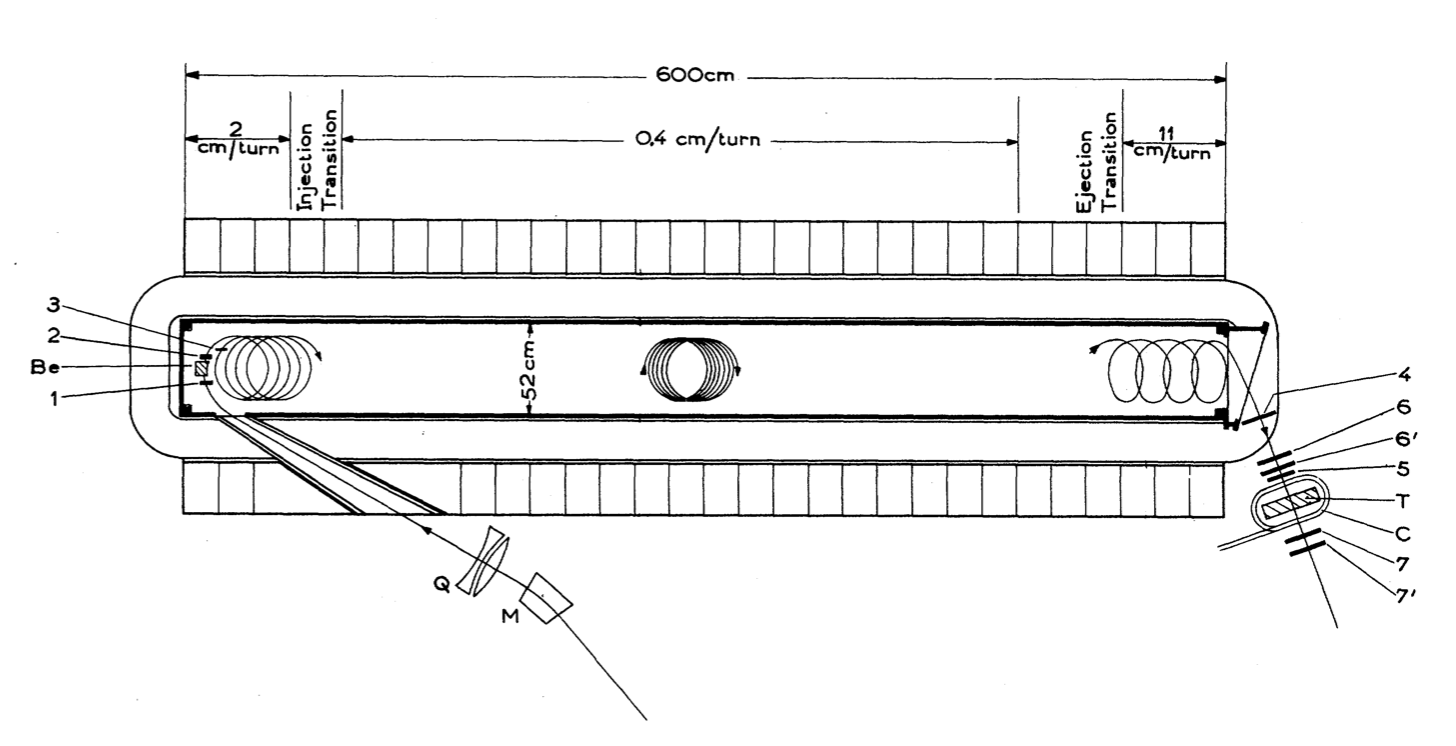
\includegraphics[width=0.9\linewidth]{fig/cern-i-diagram.png}
\label{fig:cern-i}
\caption{A diagram of the experimental setup in the first muon \gmtwo experiment at CERN. The muons enter from the lower left, go through the energy moderator to put the cyclotron radius at 19cm, drift and circles toward the ejection side of the magnetic, escape from the the magnet, stop in the fiducial block, and decay into an electron with momentum correlated to the spin direction.}
\end{figure}

The second iteration at CERN was the first muon \gmtwo to use a storage ring.



\todo{Research the CERN expts}

 of quantum field theory models of particle interactions.  Shortly after theoretical predictions placed the value of g-2 as slightly larger than $2$ due to interactions with quantum vacuum fluctuations, experimentalists were able to measure the deviation.  The phenemenon remained relevant for subsequent years, inspiring several experiments at CERN, the high precision experiment at Brookhaven Nation Lab (BNL), an independent experiment at J-PARC, and the second iteration of the BNL experiment which will soon begin at Fermi National Accelerator Laboratory (FNAL).

The most precise Muon g-2 experiment to date, took place at Brookhaven National Lab. The E821 experiment, as it is labeled in high energy physics ledgers, was groundbreaking.  The scale of the experiment rose \todo{The langugage will depend on previous sections, build in order}

\section{Motivation}



